\documentclass[]{article}
\usepackage{amsmath}
\usepackage{graphicx}
\graphicspath{.}

%opening
\title{AERO 7970 Midterm Exam}
\author{Matthew Boler}

\begin{document}

\maketitle


\section{Question 1}
Given the system:
\begin{equation}
	G(s) = \begin{bmatrix}
	\frac{10(s+1)}{s^2 + 0.2s + 100} \frac{1}{s+1} \\
	\frac{s+2}{s^2 + 0.1s + 10} \frac{5(s+1)}{(s+2)(s+3)}
	\end{bmatrix}
\end{equation}

\begin{itemize}
	\item Find a state space realization
	\item Determine the controllability and observability
	\item Find the transmission zeroes and eigenvalues of the A matrix using Matlab
	\item Find the H2 and Hinf norms and plot the Hinf vs frequency
	\item Plot the singular values vs frequency
\end{itemize}

\subsection{State Space Realization}
\noindent $G(s)$ can be split into the following transfer functions:
\begin{align}
	\frac{y_1(s)}{u_1(s)} &= \frac{10(s+1)}{s^2 + 0.2s + 100}\\
	\frac{y_2(s)}{u_1(s)} &= \frac{1}{s+1} \\
	\frac{y_1(s)}{u_2(s)} &= \frac{s+2}{s^2 + 0.1s + 10} \\
	\frac{y_2(s)}{u_2(s)} &= \frac{5(s+1)}{(s+2)(s+3)}
\end{align}

\noindent By introducing the intermediate variables $z_1 - z_4$, these can be rewritten as:
\begin{align}
	\frac{y_1}{u_1} &= \frac{10\dot{z}_1 + 10 z_1}{\ddot{z}_1 + 0.2\dot{z}_1 + 100z_1} \\
	\frac{y_1}{u_1} &= \frac{\dot{z}_2 + 2z_2}{\ddot{z}_2 + 0.1\dot{z}_2 + 10z_2} \\
	\frac{y_1}{u_1} &= \frac{z_3}{\dot{z}_3 + z_3} \\
	\frac{y_1}{u_1} &= \frac{5\dot{z}_4 + 5z_4}{\ddot{z}_4 + 5\dot{z}_4 + 6z_4}
\end{align}

\noindent By choosing $(\dot{z}_1, z_1, \dot{z}_2, z_2, z_3, \dot{z}_4, z_4)^T$ as our state variables, we arrive at the realization:

\begin{align*}
	\mathbf{A} &= \begin{bmatrix}
	-0.2 & -100 & 0 & 0 & 0 & 0 & 0 \\
	1 & 0 & 0 & 0 & 0 & 0 & 0 \\
	0 & 0 & -0.1 & -10 & 0 & 0 & 0 \\
	0 & 0 & 1 & 0 & 0 & 0 & 0 \\
	0 & 0 & 0 & 0 & -1 & 0 & 0 \\
	0 & 0 & 0 & 0 & 0 & -5 & -6 \\
	0 & 0 & 0 & 0 & 0 & 1 & 0
	\end{bmatrix} \\
	\mathbf{B} &= \begin{bmatrix}
	1 & 0 \\
	0 & 0 \\
	1 & 0 \\
	0 & 0 \\
	0 & 1 \\
	0 & 1 \\
	0 & 0
	\end{bmatrix}\\
	\mathbf{C} &= \begin{bmatrix}
	10 & 10 & 0 & 0 & 1 & 0 & 0 \\
	0 & 0 & 1 & 2 & 0 & 5 & 5
	\end{bmatrix} \\
	\mathbf{D} &= 0
\end{align*}

\subsection{Controllability and Observability}
\noindent By using $>>ctrb(A, B)$ and $>>obsv(A, C)$, we find that both the controllability and observability matrices are full rank, so the system is controllable and observable.

\subsection{Transmission Zeros and Eigenvalues}

\noindent Via $>>tzero(A, B, C, D)$, the transmission zeros of the system are:

\begin{align*}
	tz &= \begin{bmatrix}
	-0.4840 \pm 3.0020i \\
	-1.4003 \pm 0.3046i \\
	0.7523 + 0.0i
	\end{bmatrix}
\end{align*}

\noindent The eigenvalues of the A matrix are:

\begin{align*}
	eig = \begin{bmatrix}
	-0.1 \pm 9.9995i \\
	-0.05 \pm 3.1619i \\
	-1.0 + 0.0i \\
	-2.0 + 0.0i \\
	-3.0 + 0.0i
	\end{bmatrix}
\end{align*}

\subsection{H2 and Hinf Norms}

\noindent Via $>>h2norm(sys)$, the $H_2$ norm is:
\begin{align*}
	H_2 &= 16.2147
\end{align*}

\noindent Via $>>G = pck(A, B, C, D); >>hinfnorm(G)$, the $H_{\inf}$ norm is:

\begin{align*}
	H_{\inf} &= 50.2496 
\end{align*}

\subsection{Singular Values vs Frequency}

The plot of singular values vs frequency is shown below:

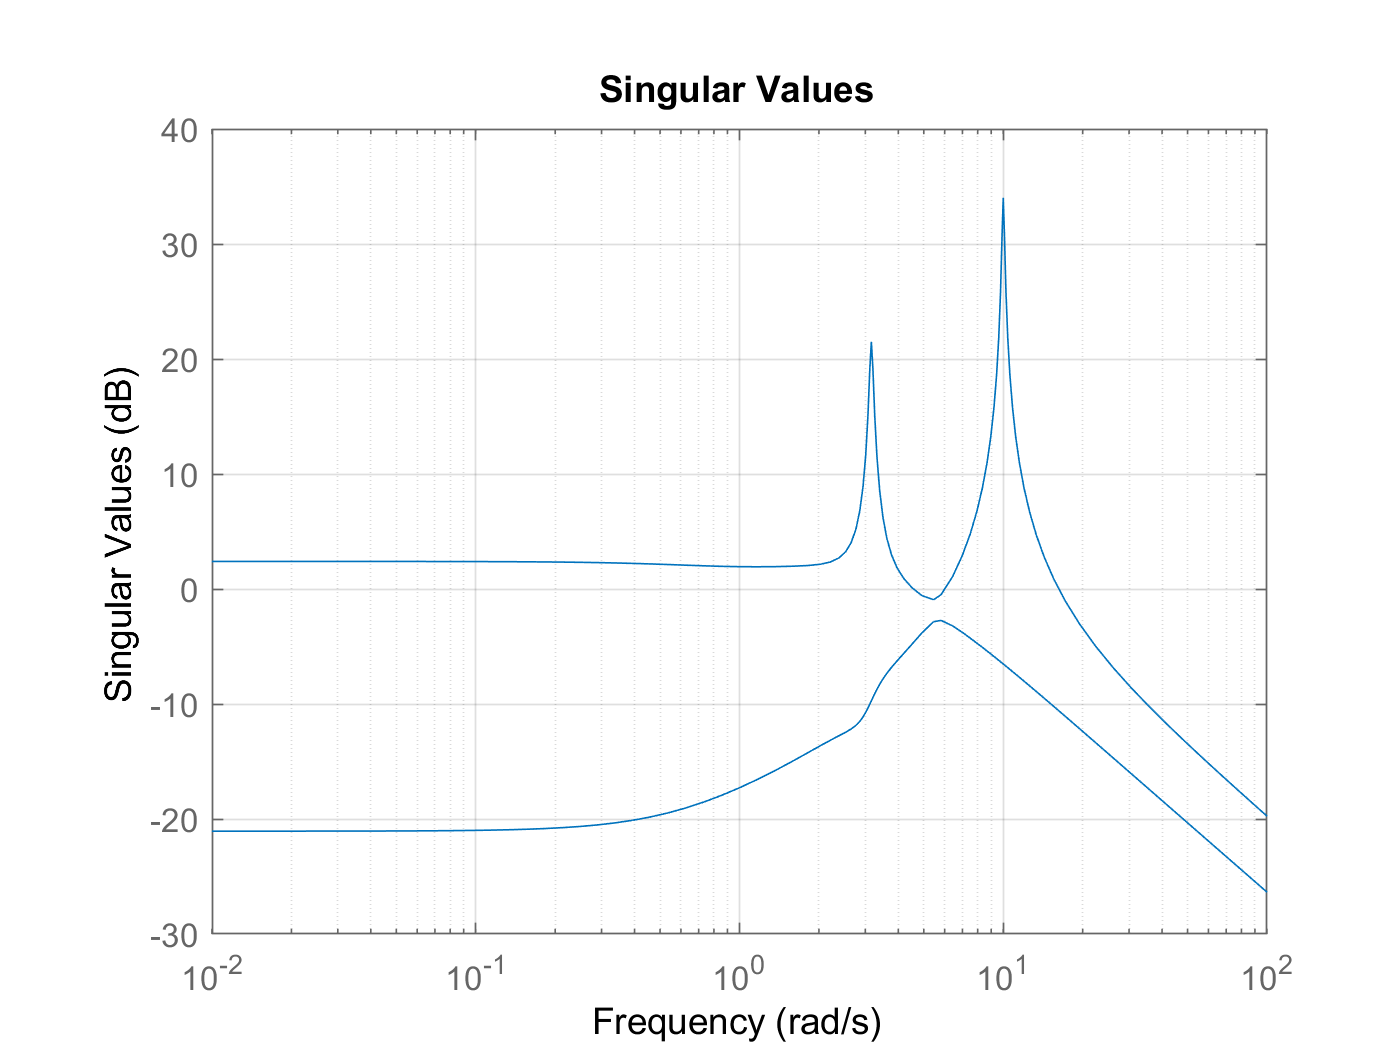
\includegraphics[width=\textwidth]{singular_values.png}



\section{Question 2}
\noindent Using the class notes and the appropriate handouts, provide a 1 page max explanation of the relationship between Hamiltonian matrices and algebraic Riccati equations, concentrating on the LQR guaranteed closed loop stability.

\subsection{Solution}

\noindent For the LQR problem, we have the associated Hamiltonian
\begin{align*}
	\textit{H} &= \begin{bmatrix}
	A & -BR^{-1}B^T \\
	-Q^T & -A^T
	\end{bmatrix}
\end{align*}
\noindent and algebraic Riccati equation:
\begin{align*}
	A^TS + SA + Q - SBR^{-1}B^TS = 0
\end{align*}

\noindent The relationship between the Hamiltonian and the ARE is fundamentally that the Hamiltonian defines a unique, stabilizing solution $S$ of the ARE (assuming a controllable and observable system), which then results in a stabilizing controller which minimizes the cost function associated with the $Q,R$ matrices (and is therefore the solution to the LQR problem).

\noindent From the theorems given in the notes and chapter 13 of the Zhou book, the logic that defines this relationship is as such:

\begin{itemize}
	\item A matrix which solves the ARE can be defined relative to a subspace of the Hamiltonian. 
	\item There can be defined two subspaces of the Hamiltonian: $X_{-}(H)$ and $X_{+}(H)$ which correspond to its negative and positive eigenvalues, respectively.
	\item A matrix $S$ which solves the ARE for $X_{-}(H)$ is unique, real symmetric, and results in a stable $A+RS$.
\end{itemize}
\noindent From these theorems, we can see that a matrix $S$ that solves the ARE can be defined relative to the subspace of the Hamiltonian which corresponds to the negative eigenvalues of the Hamiltonian, and for this matrix, the matrix $A+RS$ is stable.
As $A+RS$ is directly related to the feedback system $A-BK$, finding $S$ is equivalent to finding the desired controller $K$.

\section{Question 3}

\noindent Given the system:
\begin{align}
	G(s) &= \frac{y(s)}{r(s)} = \frac{s+1}{s+10 \pm 0.1 \delta}, |\delta| \leq 1
\end{align}

\noindent Show that it is equivalent to
\begin{align}
	P(s) &= \begin{bmatrix}
	\frac{-0.1}{s + 10} \frac{-0.1(s+1)}{s(s+1)} \\
	\frac{1}{s+10} \frac{s+1}{s(s+10)}
	\end{bmatrix} \\
	\begin{bmatrix}
	z \\
	y
	\end{bmatrix} &= P(s) \begin{bmatrix}
	p \\
	r
	\end{bmatrix}	
\end{align}

\noindent We split $P(s)$ into its component equations:
\begin{align}
	\frac{y(s)}{p(s)} &= \frac{1}{s+10} \\
	\frac{y(s)}{r(s)} &= \frac{s+1}{s(s+10)} \\
	\frac{z(s)}{p(s)} &= \frac{-0.1}{s + 10} \\
	\frac{z(s)}{r(s)} &= \frac{-0.1(s_10)}{s(s+10)} 
\end{align}

\noindent Recognizing that this is an upper fractional transformation, we apply:
\begin{align*}
	F(M,\Delta) &= M_{22} + M_{21}\Delta(I-M_{11}\Delta)^{-1}M_{12} \\
	&= \frac{s+1}{s(s+10)}+\frac{s+1}{s(s+10)}\Delta(1-\frac{0.1\Delta}{s+10})^{-1}\frac{-0.1(s+1)}{s(s+10)}\\
	&= \frac{s+1}{s+10} + \frac{-0.1\Delta(s+1)}{s(s+10)(s+10+0.1\Delta)} \\
	&= \frac{(s+1)(s+10+0.1\Delta)}{s(s+10)(s+10+0.1\Delta)} + \frac{-0.1\Delta(s+1)}{s(s+10)(s+10+0.1\Delta)} \\
	&= \frac{s+1}{s(s + 10 + 0.1\Delta)}
\end{align*}

\noindent which is equivalent to the given system with the exception of an extra integrator.



\end{document}
